%%%%%%%%%%%%%%%%%%%%%%%%%%%%%%%%%%%%%%%%%%%%%%%%%%%%%%%%%%%
% Electronic Journal of Mathematics and Technology (eJMT) %
% style sheet for LaTeX.  Please do not modify sections   %
% or commands marked 'eJMT'.                              %
%                                                         %
%%%%%%%%%%%%%%%%%%%%%%%%%%%%%%%%%%%%%%%%%%%%%%%%%%%%%%%%%%%
%                                                         %
% eJMT commands                                           %
%                                                         %
\documentclass[12pt,a4paper]{article}%                    %
\usepackage{times}                                        %
\usepackage{amsfonts,amsmath,amssymb}                     %
\usepackage[a4paper]{geometry}                            %
\usepackage{fancyhdr}                                     %
\usepackage{color}                                        %
\usepackage[pdftex]{hyperref} % see note below            %
\usepackage{graphicx}%                                    %
\hypersetup{                                              %
    a4paper,                                              %
    breaklinks                                            %
}                                                         %
%                                                         %
\newtheorem{theorem}{Theorem}                             %
\newtheorem{acknowledgement}[theorem]{Acknowledgement}    %
\newtheorem{algorithm}[theorem]{Algorithm}                %
\newtheorem{axiom}[theorem]{Axiom}                        %
\newtheorem{case}[theorem]{Case}                          %
\newtheorem{claim}[theorem]{Claim}                        %
\newtheorem{conclusion}[theorem]{Conclusion}              %
\newtheorem{condition}[theorem]{Condition}                %
\newtheorem{conjecture}[theorem]{Conjecture}              %
\newtheorem{corollary}[theorem]{Corollary}                %
\newtheorem{criterion}[theorem]{Criterion}                %
\newtheorem{definition}[theorem]{Definition}              %
\newtheorem{example}[theorem]{Example}                    %
\newtheorem{exercise}[theorem]{Exercise}                  %
\newtheorem{lemma}[theorem]{Lemma}                        %
\newtheorem{notation}[theorem]{Notation}                  %
\newtheorem{problem}[theorem]{Problem}                    %
\newtheorem{proposition}[theorem]{Proposition}            %
\newtheorem{remark}[theorem]{Remark}                      %
\newtheorem{solution}[theorem]{Solution}                  %
\newtheorem{summary}[theorem]{Summary}                    %
\newenvironment{proof}[1][Proof]{\noindent\textbf{#1.} }  %
{\ \rule{0.5em}{0.5em}}                                   %
%                                                         %
% eJMT page dimensions                                    %
%                                                         %
\geometry{left=2cm,right=2cm,top=3.2cm,bottom=4cm}        %
%                                                         %
% eJMT header & footer                                    %
%                                                         %
\newcounter{ejmtFirstpage}                                %
\setcounter{ejmtFirstpage}{1}                             %
\pagestyle{empty}                                         %
\setlength{\headheight}{14pt}                             %
\geometry{left=2cm,right=2cm,top=3.2cm,bottom=4cm}        %
\pagestyle{fancyplain}                                    %
\fancyhf{}                                                %
\fancyhead[c]{\small The Electronic Journal of Mathematics%
\ and Technology, Volume 1, Number 1, ISSN 1933-2823}     %
\cfoot{%                                                  %
  \ifnum\value{ejmtFirstpage}=0%                          %
    {\vtop to\hsize{\hrule\vskip .2cm\thepage}}%          %
  \else\setcounter{ejmtFirstpage}{0}\fi%                  %
}                                                         %
%                                                         %
%%%%%%%%%%%%%%%%%%%%%%%%%%%%%%%%%%%%%%%%%%%%%%%%%%%%%%%%%%%
%
% Please place your own definitions here
%
\def\GEONExT{GEONE\kern-.06em \lower.5ex\hbox{x}\kern-.215em T}
%
%%%%%%%%%%%%%%%%%%%%%%%%%%%%%%%%%%%%%%%%%%%%%%%%%%%%%%%%%%%
%                                                         %
% How to use hyperref                                     %
% -------------------                                     %
%                                                         %
% Probably the only way you will need to use the hyperref %
% package is as follows.  To make some text, say          %
% "My Text Link", into a link to the URL                  %
% http://something.somewhere.com/mystuff, use             %
%                                                         %
% \href{http://something.somewhere.com/mystuff}{My Text Link}
%                                                         %
%%%%%%%%%%%%%%%%%%%%%%%%%%%%%%%%%%%%%%%%%%%%%%%%%%%%%%%%%%%
%
\begin{document}
%
% document title
%
\title{JSXGraph -- Dynamic Mathematics Running on (nearly) Every Device}%
%
% Single author.  Please supply at least your name,
% email address, and affiliation here.
%
\author{\begin{tabular}{c}
\textit{Michael Gerh\"auser, Bianca Valentin, Alfred Wassermann, Peter Wilfahrt} \\
alfred.wassermann@uni-bayreuth.de\\
Department of Mathematics, 
University of Bayreuth\\
95440 Bayreuth, 
Germany\end{tabular}
}%
%
%%%%%%%%%%%%%%%%%%%%%%%%%%%%%%%%%%%%%%%%%%%%%%%%%%%%%%%%%%%
%                                                         %
% eJMT commands - do not change these                     %
%                                                         %
\date{}                                                   %
\maketitle                                                %
%                                                         %
%%%%%%%%%%%%%%%%%%%%%%%%%%%%%%%%%%%%%%%%%%%%%%%%%%%%%%%%%%%
%
% abstract
%
\begin{abstract}
%
JSXGraph is a stand-alone library for displaying dynamic mathematics, e.g. dynamic geometry, 
function plotting, turtle graphics, and much more, in a web browser. 
It is written in JavaScript and runs on a broad variety of devices from 
desktop computers down to smart-phones and tablet computers. 

JSXGraph is able to import various file formats like \GEONExT{}, GeoGebra, Intergeo, 
and---at least partially---Cinderella. Further, it provides a proramming
interface (API) for the development of mathlets, i.e. special
purpose programs to visualize mathematics.
At the moment, JSXGraph is the only software for dynamic mathematics, which
supports the whole range of computers from Desktop computers
downto tablet computers and smart-phones.
%
\end{abstract}%
%
%%%%%%%%%%%%%%%%%%%%%%%%%%%%%%%%%%%%%%%%%%%%%%%%%%%%%%%%%%%
%                                                         %
% eJMT command                                            %
%                                                         %
\thispagestyle{fancy}                                     %
%                                                         %
%%%%%%%%%%%%%%%%%%%%%%%%%%%%%%%%%%%%%%%%%%%%%%%%%%%%%%%%%%%
%
% Please use the following to indicate sections, subsections,
% etc.  Please also use \subsubsection{...}, \paragraph{...}
% and \subparagraph{...} as necessary.
%



\section{Introduction}
In the late 1990s the availability of graphical web browsers that enabled easy access to the 
World Wide Web 
brought many fresh ideas to the class room and to mathematics education. 
The programming language Java became the dominant tool to raise interactivity in 
dynamic mathematics to a new level. Countless new Java based \emph{Mathlets} came to existence 
to visualize many aspects of mathematics with levels varying from Kindergarten to University. 
Also, powerful software systems were developed that combined geometry and calculus 
under one graphical user interface. The most prominent examples are 
Cinderella~\cite{kortenkamp1999}, \GEONExT~\cite{ehmann2003} and GeoGebra~\cite{hohenwarter2005} 
to name a few of them.
Also, desktop programs are of importance. Examples are
{\sl The Geometer's Sketchpad}\footnote{\href{http://www.dynamicgeometry.com}{http://www.dynamicgeometry.com}} 
and {\sl Cabri II plus}\footnote{\href{http://cabri.com}{http://cabri.com}}, 
both available for Windows and MacOS.

But now a new hardware generation is on the horizon which appears to be better suited 
for the class room than the old clumsy Personal Computer. 
The revolution started with the success of small and cheap netbooks and the appearance of 
powerful smart-phones. 
Now, these two complementary worlds seem to melt together into tablet computers. 
The success of the iPad by Apple confirms this. 
Probably, very soon many other hardware manufacturer will follow and produce 
cheaper tablet computers having more features than the iPad.

Now, mathematics education faces the challenge that most of the existing web-based software 
for dynamic mathematics is implemented in Java and embedded in web pages as so called Java applets.  
But there will be no Java plug-in available on most of these new machines. 
Without good software the new hardware is useless for learning mathematics 
in the class room.

With the project JSXGraph\footnote{\href{http://jsxgraph.org}{http://jsxgraph.org}} 
at the University of Bayreuth we tried to take up 
this challenge and offer first class dynamic mathematics software that runs on 
every device including smart-phones, netbooks, tablet computers and Desktop PCs. 
Moreover, the goal is to provide compatibility for existing resources for 
mathematics education. 

JSXGraph is a free software library for mathematical visualizations in a web browser.
Its feature set covers {\sl dynamic Geometry}, plotting of {\sl function graphs} and
{\sl curves} of various types, {\sl charts}, and {\sl turtle graphics}

Usually, JSXGraph is embedded in web pages, for on- or off\/line viewing.
The download size is a mere 80 kByte, when embedded in web pages.
JSXGraph enhanced web pages can be viewed with all major web browsers 
on nearly every hardware platform and operating system.
The supported hardware ranges from smartphones and tablet computers 
running iOS or Android to Desktop PC running Windows, MacOS X or Linux.

At the time of writing, JSXGraph is the only dynamic geometry system that runs  
on such a broad range of  devices and web browsers---without installation of any plug-in 
or wathsoever additional software.
JSXGraph is usable even on devices with limited computing resources, 
like older Desktop PCs running Microsoft Internet Explorer 6.0. 

Thus, this library may prove to be helpful for the
introduction of technology in mathematical education in developing countries.

\section{Computers in mathematics education}
As of today three types of computers are used by students in class room:
\begin{itemize}
\item Desktop PC: high computing power, runs desktop programs and web based software, 
the web browser contains Java plug-in and Flash plug-in, robust hardware,
requires computer lab, need power plug, expensive.
\item Programmable Desktop Calculator: low computing power, low graphical resolution, runs only
special purpose software, no web access, no computer lab necessary, long battery life, 
very robust hardware, cheap.
\item Laptop, netbook: medium to high computing power, no computer lab necessary, 
medium to long battery life, software like Desktop PC, but Java plug-in may not be available, or maybe slow,
medium priced to expensive, fragile hardware.
\end{itemize}
Soon, the new generation of tablet computers will be available and these devices will be
well suited for the classs room: cheap to medium priced, robust hardware, medium
computing power, long battery life, running desktop special purpose programs and web based software,
Java plug-in is not available, Flash plug-in may be available.

The tablet computers seem to combine the advantages of the Programmable Desktop Calculator 
and the laptop. 

The most notable disadvantages of these devices are that typing is still not as easy 
as with a physical keyboard and that none of the available software for 
dynamic mathematics is available for these platforms.

The situation for implementors of dynamic mathematics software is difficult because there exists a variety
of different hardware and software platforms used by these devices. Thus, 
web-based software seems to be the only managable solution to provide 
dynamic mathematics software for all platforms simultaneously.

\section{Background on web based visualization}\label{sec:3}
For implementing dynamic mathematics software for the web browser for all platforms 
the only possible programming language is JavaScript~\cite{crockford}. In the first years of its availability
JavaScript was running very slow, but recently the browsers come with very advanced
Just-in-Time compilers for JavaScript. Moreover, the initalisation time of a 
JavaScript program is close to zero in contrast to some Java plug-ins, see the online versions of
Figures~\ref{fig:geonext}, \ref{fig:geogebra}, and \ref{fig:cindy}.

For realizing graphical output in the web browser 
that can be manipulated by JavaScript there are several possibilities,
depending on the browser:
\begin{itemize}
\item SVG:\footnote{\href{http://www.w3.org/TR/SVG/}{http://www.w3.org/TR/SVG/}}
Scalable Vector Graphics, vector graphics format.
\item VML:\footnote{\href{http://www.w3.org/TR/NOTE-VML}{http://www.w3.org/TR/NOTE-VML}}
Vector Markup Language,  vector graphics format.
\item Canvas:\footnote{\href{https://developer.mozilla.org/en/Canvas_tutorial}{https://developer.mozilla.org/en/Canvas\_tutorial}}
bitmap graphics.
\end{itemize}
\begin{table}
\begin{center}
\begin{tabular}{c*{7}{|c}}
    & Firefox 3+ & \multicolumn{2}{c|}{Internet Explorer} & Opera & Safari        & \multicolumn{2}{c}{Chrome} \\
    &            &      4-8         & 9                  &      & incl. iPad & Desktop          & Android $\leq2.2$\\
\hline 
SVG &  \checkmark   &  --           &  \checkmark     &  \checkmark   &  \checkmark   &  \checkmark   &     --    \\
VML &      --       &  \checkmark   &  \checkmark     &     --        &     --        &     --        &     --         \\
Canvas & \checkmark & --            &  \checkmark     &  \checkmark   &  \checkmark   &  \checkmark   &  \checkmark    \\
\hline
market share &  22.93\% & 60.4\%    & --              &  2.37\%       &   5.16\%      &  \multicolumn{2}{c}{7.52\%} \\ 
\end{tabular}
\caption{Supported graphics formats of the most popular web browsers. The market share data
is from August 2010, see~\cite{netapplications}.}\label{table:1}
\end{center}
\end{table}
Table~\ref{table:1} shows that if a software wants to support graphical output on all 
major web browsers then it has to support at least the canvas element and VML. 
In the context of dynamic geometry, the SVG format -- if available -- seems to be 
slightly better suited than the canvas element, see~\cite{kaipiainen}.

For tablet computers Safari and the Android version of Chrome will most likely become the
predominant browsers, since many of these devices are announced to be based on Android.
For a future release of Android, SVG support of Chrome has been announced.

Even with the availability of the Internet Explorer 9 the need for support of
VML will remain for some years, because Internet Explorer 9 will not be available 
on older machines running Windows XP.
This seems to be especially the case for schools and public institutions which are
typically slow on updating their computing infrastructure. 
The slow adaption rate is also underpinned by the survey~\cite{netapplications} which
shows that in August 2010 the Internet Explorer 6 still had a market share of 16.18\%
despite the availability of versions 7 and 8 since some years.


\section{The library JSXGraph for dynamic mathematics}
The open-source library JSXGraph, developed at the University of Bayreuth, 
addresses the above problems.
JSXGraph is a pure JavaScript implementation, it does not rely on any other 
library. By default, JSXGraph uses the vector graphic format SVG
for graphical output in a web browser. If SVG is not available it falls
back to either VML or canvas.

Another pure JavaScript implementation of a Dynamic Geometry system is
GeometryEditor\footnote{\href{http://wme.cs.kent.edu/geosvg/}{http://wme.cs.kent.edu/geosvg/}}, 
formerly known as GeoSVG. But there, the graphical output is restricted to SVG.

First publicly presented in 2008~\cite{ehmann2008}, JSXGraph offers all 
functionality of Dynamic Geometry System (DGS), including conic sections.
Meanwhile, the features of JSXGraph go far beyond the possibilities
of most DGS.
The following list gives an overview of possibilities of JSXGraph.

\begin{description}
\item[Geometry elements:]
point, glider, intersection, parallel, perpendicular,
line, segment, axis, tangent, normal, vector,
circle, circumcircle, ellipse, hyperbola, parabola, conic defined by five points,
polygon, regular polygon, 
midpoint, mirror point, reflection point, 
semicircle, circumcircle arc, circumcircle sector,
angle, bisector, bisector lines,
exact loci computation, homogeneous and affine coordinates
\item[Calculus:]
function graph, parametric curve, polar plot, 
Lagrange interpolation, cubic spline, B-spline, Bezier curve,
regression polynomials of arbitrary degree, 
Riemann sums, 
numerical differentiation, numerical integrations,
numerical solution of systems of ordinary differential equations,
matrix computions, root finding,
Eigenvalues, -vectors
\item[Charts:]
bar chart, line chart, point chart, radar chart, cartogram
\item[Other:]
slider, images, 
projective transformation, turtle graphics, various types of animation,
various R-like statistical functions, Lindenmayer systems
\item[Display options:]
HSV color palette, shadows, dynamic texts with \LaTeX{}-support 
via MathJax\footnote{\href{http://mathjax.org}{http://mathjax.org}}, 
flexible layers
\end{description}
The goal of JSXGraph is to be real dynamic. For example, 
the degree of a regression 
polynomial\footnote{\href{http://jsxgraph.uni-bayreuth.de/wiki/index.php/Polynomial_regression_I}{http://jsxgraph.uni-bayreuth.de/wiki/index.php/Polynomial\_regression\_I}} 
or the fill color of certain 
elements\footnote{\href{http://jsxgraph.uni-bayreuth.de/wiki/index.php/Infinity}{http://jsxgraph.uni-bayreuth.de/wiki/index.php/Infinity}} 
may depend on other elements.

The  size 
of the JSXGraph code is about 380 kByte. If the web server delivering the 
content has data compression enabled (which should be the default anyhow) the 
size of the transmitted code is about 80 kByte. To compare it with Java software, 
for example the size of the \GEONExT{} archive is about 1 Mbyte. 

In order to use JSXGraph 
the web developer has to include only two files in the 
HTML file: the JSXGraph code and a CSS file. 
JSXGraph 
is released under the Lesser GNU General Public License (LGPL), the source code
is available at Sourceforge\footnote{\href{http://sourceforge.net/projects/jsxgraph/}{http://sourceforge.net/projects/jsxgraph/}}.

As explained in Section~\ref{sec:3}, JSXGraph runs on every hardware and operating system which has a graphical 
web browser. 
All the mainstream web browser are supported, Firefox 3+, Internet Explorer
6+ (including the upcoming version 9), Google Chrome (all versions). 
The browsers Safari, Opera are supported since at least 2008. 
The range of supported hardware thus reaches from Desktop PCs 
down to tablet computers and smartphones. 

With JSXGraph it is possible to access modern mathematical content even with old computers
running Internet Explorer 6.
But even on more powerful computers JSXGraph has the advantage over Java based software 
that the downloading time and the initialization time is much shorter than for comparable Java applets. 

In summary, JSXGraph is usable on a huge amount of devices and should be able to take up the challenge and support dynamic mathematics on the upcoming hardware generation.
At the time of writing, there is no other software for dynamic mathematics that can be used on such a wide range of 
platforms.


\section{JSXGraph as DGS viewer}
JSXGraph is able to read and display the following file formats:
\begin{itemize} 
\item \GEONExT{}\footnote{\href{http://geonext.org}{http://geonext.org}}
\item Intergeo\footnote{\href{http://i2geo.eu}{http://i2geo.eu}}
\item GeoGebra\footnote{\href{geogebra.org}{http://geogebra.org}}
\item Cinderella\footnote{\href{http://cinderella.de}{http://cinderella.de}}
\end{itemize}
The support of the \GEONExT{} file format~\cite{ehmann2003,ehmann2008} by JSXGraph is close to 100\%. 
Only very few \GEONExT{} resources are misinterpreted by JSXGraph. 
In Figure~\ref{fig:geonext} the construction to the right is the \GEONExT{} Java applet, to the left is the same file displayed by JSXGraph.
\begin{figure}[ht]
\begin{center}
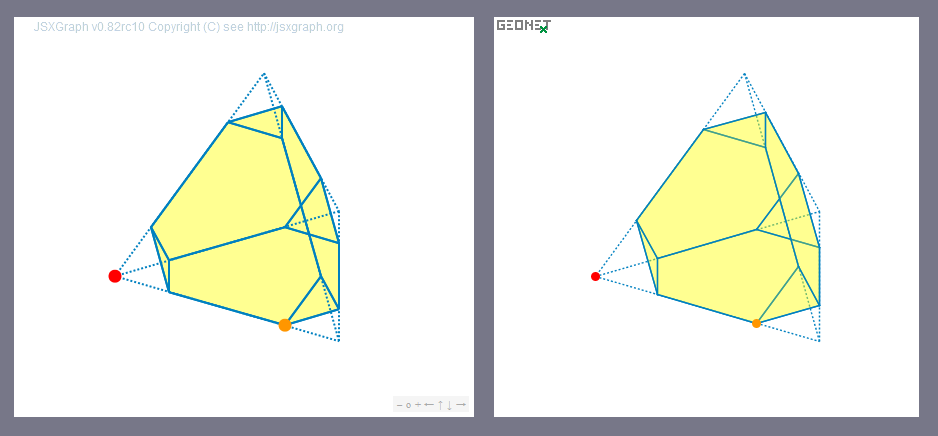
\includegraphics[width=0.8\textwidth]{geonext.png}\\
\caption{The right image shows a \GEONExT{} Java applet, 
the left image contains the same construction displayed 
by JSXGraph
(\href{http://jsxgraph.uni-bayreuth.de/talks/cadgme10/talk/jsx_gxt.html}{online version}).}\label{fig:geonext}
\end{center}
\end{figure}

The Intergeo~\cite{kortenkamp2009} format is an upcoming common file format supported by the most European implementors of dynamic geometry systems. JSXGraph possesses one of the most complete implementations of the file formats. At the time of writing, the file format just starts to gain popularity. 

\begin{figure}[ht]
\begin{center}
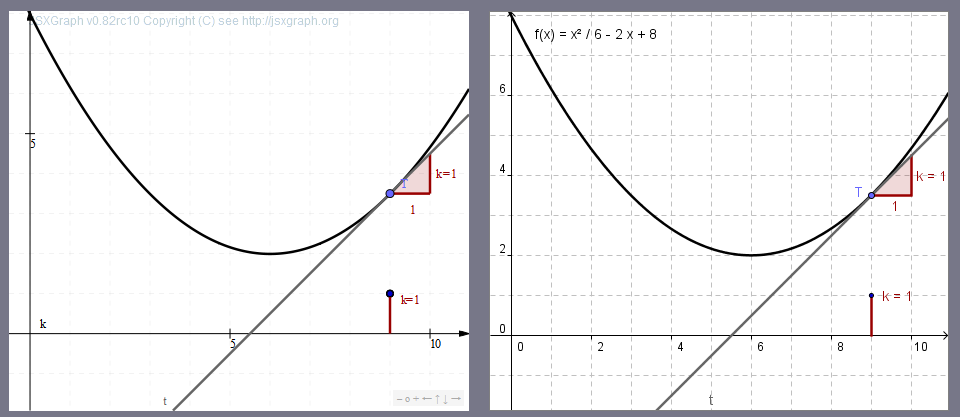
\includegraphics[width=0.8\textwidth]{geogebra.png}\\
\caption{The right image shows a GeoGebra Java applet, 
the left image contains the same construction displayed 
by JSXGraph
(\href{http://jsxgraph.uni-bayreuth.de/talks/cadgme10/talk/jsx_ggb.html}{online version}).}\label{fig:geogebra}
\end{center}
\end{figure}
The support of the GeoGebra file format~\cite{hohenwarter2005} is not complete, 
but covers the most common features of GeoGebra. 
In Figure \ref{fig:geogebra} the construction to the right is the GeoGebra Java applet, 
to the left is the same file displayed by JSXGraph.


\begin{figure}[ht]
\begin{center}
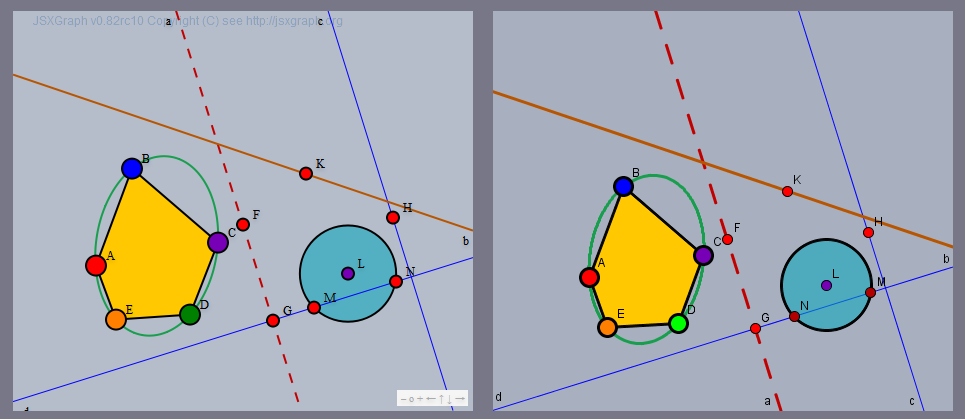
\includegraphics[width=0.8\textwidth]{cindy.png}\\
\caption{The right image shows a Cinderella Java applet, 
the left image contains the same construction displayed 
by JSXGraph 
(\href{http://jsxgraph.uni-bayreuth.de/talks/cadgme10/talk/jsx_cdy.html}{online version}).}\label{fig:cindy}
\end{center}
\end{figure}
The support of the Cinderella file format \cite{kortenkamp1999} by JSXGraph is in a very early development stage. At the moment it comprises most of the Euclidean Geometry part of Cinderella. In Figure~\ref{fig:cindy} the construction to the right is the Cinderella Java applet, to the left is the same file displayed by JSXGraph.


\section{Constructing with JessieScript}
JSXGraph comes with a simple geometric construction language called JessieScript, which is closely related to the syntax students use in school to describe their construction by compass and ruler. An example is shown in Figure~\ref{fig:jessiescript}, the online version is available at 
\href{http://jsxgraph.uni-bayreuth.de/jessie}{http://jsxgraph.uni-bayreuth.de/jessie}. 
The whole web page consists of three elements: the form for the text input of the construction, the display of the construction and a log window. 
Another side effect of JessieScript is security. In the web application of Figure~\ref{fig:jessiescript}
input is restricted to 
JessieScript syntax, all other input is ignored. This makes it difficult to 
infiltrate malicious JavaScript code.
\begin{figure}[ht]
\begin{center}
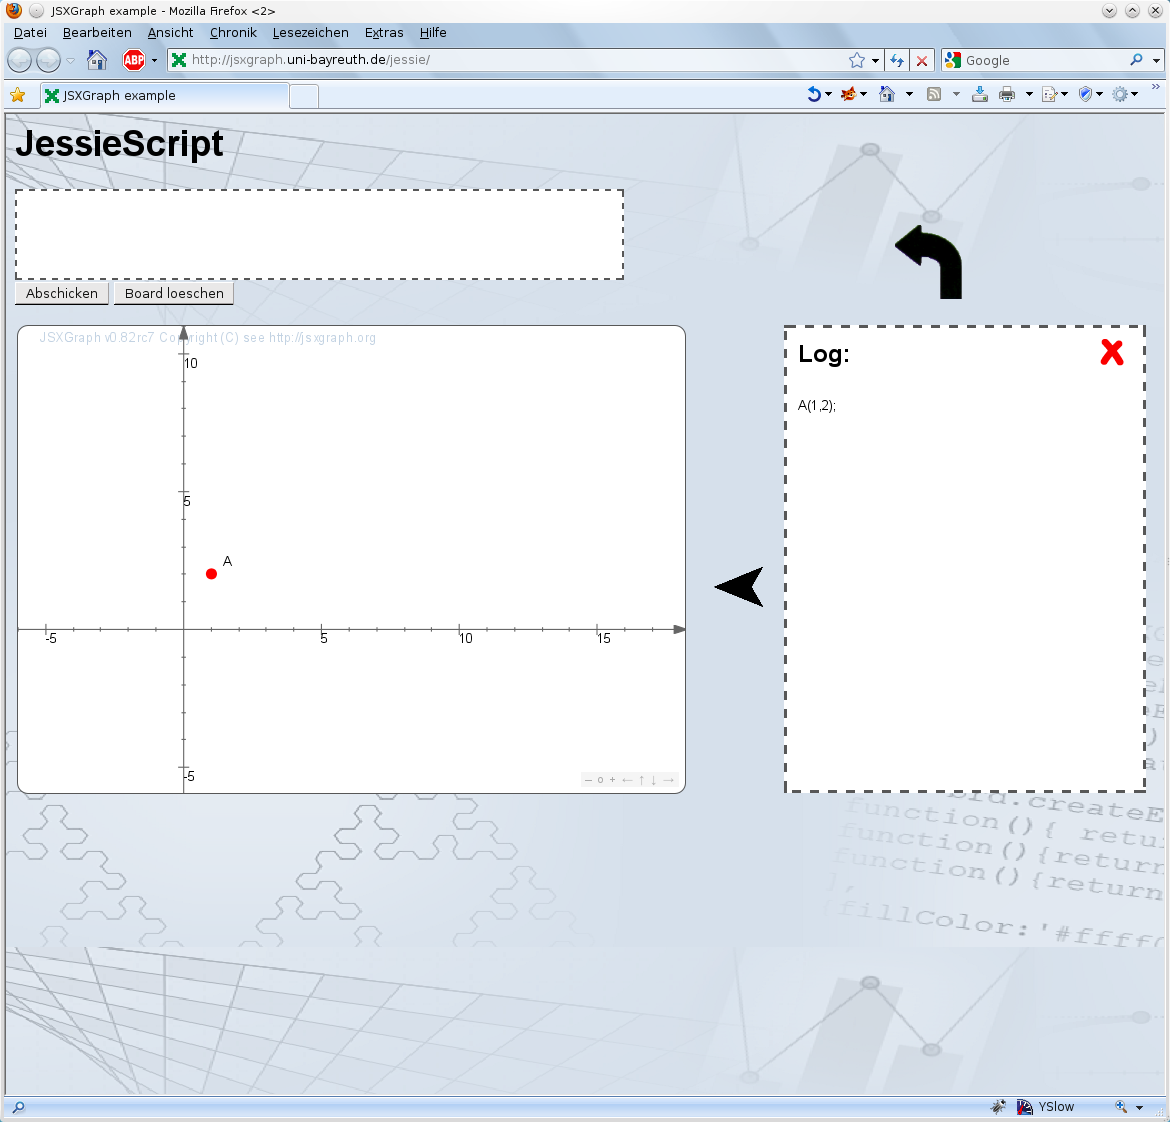
\includegraphics[width=0.8\textwidth]{jessiescript.png}\\
\caption{A simple web page for constructiong with JessieScript 
(\href{http://jsxgraph.uni-bayreuth.de/jessie/}{online version}).}\label{fig:jessiescript}
\end{center}
\end{figure}

The most important JessieScript commands are:
\begin{description}
\item{-- \verb+A(1,1)+:} Point with name '\verb|A|' at position $(1,1)$
\item{-- \verb+ZY(0.5|1)+:} Point with name '\verb|ZY|' at position $(0.5,1)$
\item{-- \verb|]AB[|:} straight line through points $A$ and $B$
\item{-- \verb|[AB[|:} ray through points $A$ and $B$, stopping at $A$
\item{-- \verb|]AB]|:} ray through points $A$ and $B$, stopping at $B$
\item{-- \verb|[AB]|:} segment through points $A$ and $B$
\item{-- \verb|g=[AB]|:} segment through points $A$ and $B$, named by '\verb|g|'
\item{-- \verb|k(A,1)|:} circle with center $A$ and radius $1$
\item{-- \verb|k(A,B)|:} circle with center $A$ through point $B$ on the circle line
\item{-- \verb|k(A,[BC])|:} circle with center $A$ and radius defined by the length of the 
(not necessarily existing) segment \verb|[BC]|
\item{-- \verb|k_1=k(A,1)|:} circle with center $A$ and radius $1$, named by '\verb|k_1|' 
\end{description}
The \href{http://jsxgraph.uni-bayreuth.de/wiki/index.php/Geometric_constructions_with_JessieScript}{JessieScript wiki page} contains the full description of the syntax.


\section{Developing Mathlets with JSXGraph}
With JSXGraph it is possible to create special purpose programs for mathematics visualizations.
These are sometimes called {\sl mathlets}\footnote{See for example
\href{http://math.mit.edu/mathlets/}{http://math.mit.edu/mathlets/}}.

JSXGraph provides an API (application programming interface) to build JavaScript based 
dynamic mathematics applications for the web browser. 
The \href{http://jsxgraph.uni-bayreuth.de/wiki/index.php/Differential_equations}{differential equation plotter}
in the JSXGraph wiki is one example for using JSXGraph in mathematics 
education on the university level. 
Other applications are 
\href{http://jsxgraph.uni-bayreuth.de/wiki/index.php/Even_simpler_function_plotter}{function plotting}, 
\href{http://jsxgraph.uni-bayreuth.de/wiki/index.php/Programming_turtle_graphics}{turtle graphics}, 
and support for various possibilities to create 
\href{http://jsxgraph.uni-bayreuth.de/wiki/index.php/Category:Charts}{charts}. 
This may be especially interesting for publisher of e-books or provider of e-learning 
content. 
Further, communication between JSXGraph and special purpose software on server side is very simple, see 
Section~\ref{sec:loci} for an advanced example.


JSXGraph meanwhile is used in situations that are different 
from mathematics education, like 
\href{http://www.rhok.org/2010/06/rhok-1-0-washington-d-c-winning-hack-chasm/}{landslide prediction}. 

The \href{http://jsxgraph.uni-bayreuth.de/wiki}{JSXGraph wiki} 
contains more than 170 examples for dynamic mathematics, 
covering many areas like charts, function plotting, calculus, geometry, and turtle graphics.

For some wide-spread content management systems there exist plug-ins to ease the integration
of JSXGraph code. 
At the moment, plug-ins exist for drupal, mediawiki, moodle, and wordpress. 
For example, the code to include JSXGraph code into a wiki page powered by mediawiki with JSXGraph plug-in installed
looks the following (\href{http://jsxgraph.uni-bayreuth.de/wiki/index.php/MediaWiki_example}{online version}):

{\footnotesize
\begin{verbatim}
<jsxgraph width="500" height="500">
  var brd = JXG.JSXGraph.initBoard('jxgbox',{boundingbox:[-2,2,2,-2]});
  var p = brd.create('point',[1.5,1.5],{face:'o', size:8});
  var q = brd.create('point',[-1,-0.5],{face:'x', size:5});
  brd.create('segment',[p,q],{dash:3});
</jsxgraph>
\end{verbatim}}
The plug-in introduces the new tag name \verb|<jsxgraph>| which is an HTML \verb|<div>| element
containing the JSXGraph construction.


\section{Server side calculations}\label{sec:loci}

JSXGraph also includes a math library which provides an interface to some basic algorithms like linear equation and ode
solvers. The speed of JavaScript interpreters in modern web browsers is sufficient for small to medium sized problems
being calculated with pure JavaScript. More complex problems can be handled by JSXGraph by swapping the calculation from
the web browser to the web server. This way even existing software solutions like computer algebra systems or numerical
libraries can be used and integrated in JSXGraph.

To accomplish this, a web development technique called AJAX is used. This technique is usually used to exchange data
with a web server without reloading the whole web page. Unfortunately this comes with a lot of programming overhead
required for every JSXGraph mathlet which requires server side calculations: AJAX invocation, parsing data from JSXGraph
on the web server, formatting the output data on the server and back in the browser one has to parse the results. In
short: a whole communication protocol has to be designed and implemented. To avoid this and save the creators of JSXGraph
based worksheets this repeating and extra work, JSXGraph provides a simple yet powerful server-client-framework.

This framework is Python\footnote{\href{http://python.org/}{http://python.org/}} based on the server side and is
organized in modules. A module is loaded by a simple function call:

\begin{verbatim}
JXG.Server.load('fft');
\end{verbatim}

This sends a request to the server to load the modules fft.py, which in this case provides some methods to calculate
fourier transforms using NumPy\footnote{\href{http://numpy.scipy.org/}{http://numpy.scipy.org/}}. If the module can be
found it is loaded and answers with a list of available methods and data elements which are then integrated in JSXGraph.
From now on, all the methods provided by the module can be used as if they were JavaScript functions.

Another example of a JSXGraph server module is the \emph{loci computation}. This module is based on an algorithm
developed by \cite{botana} based on ideas first mentioned in \cite{recio}. It usually takes two points as its input: One
dependent point which is connected to a \emph{glider} by a geometric construction. A glider is a point that is bound to
an algebraic curve. First from all points of the construction the points that are required to calculate the locus are
filtered. Then JSXGraph generates a polynomial ideal and sends the ideal to the server. On the server
CoCoA\footnote{\href{http://cocoa.dima.unige.it/}{http://cocoa.dima.unige.it/}} is used to calculate the elimination ideal
which is then analyzed using matplotlib\footnote{\href{http://matplotlib.sourceforge.net/}{http://matplotlib.sourceforge.net/}}.
In a last step JSXGraph displays the locus based on the data points the server sent.

\section{Conclusion}
JSXGraph enables the usability of mathematical resources on a broad variety of 
platforms including new small tablet computers and old, outdated Desktop PCs. 
These tablet devices seem to be very well suited for use in class room, 
but up to now there is a lack of good mathematical software, since Java applets are not longer supported. 
The goal of JSXGraph is to change this situation. 

\begin{thebibliography}{99}
    \bibitem{crockford} Crockford D., \emph{JavaScript: The good parts}, Sebastopol, CA, O'Reilly (2008).
    
    \bibitem{ehmann2003} Ehmann, M., Miller, C.: ``Dynamic Mathematics with \GEONExT.''
        (Part I: The Interplay between Geometry, Algebra and Calculus)
        in: T. Triandafillidis, K. Hatzikiriakou (Editors): \emph{Technology in Mathematics Teaching}
        Proceedings of the 6th International Conference, University of Thessaly, Volos - Greece, (2003).
 
    \bibitem{ehmann2008} Ehmann, M., Miller, C., Wassermann, A.: 
        ``\href{http://jsxgraph.uni-bayreuth.de/talks/jsxgraphMathematical_and_Scientific_e-Contents.pdf}{Dynamic Mathematics with \GEONExT{}: New Concepts}''. 
        \emph{Book of Abstracts, 4th European Workshop on Mathematical \& Scientific e-Contents}
        (2008).   

    \bibitem{hohenwarter2005} Hohenwarter, M., Fuchs, K.: 
        ``Combination of Dynamic Geometry, Algebra and Calculus in the Software System GeoGebra''.  
        In: \emph{Computer Algebra Systems and Dynamic Geometry Systems in Mathematics Teaching Conference 2004}, 
        Pecs, Hungary (2005).

    \bibitem{kaipiainen} Samuli Kaipiainen, Matti Paksula: 
           ``SVG vs. Canvas on Trivial Drawing Application'', \emph{SVG Open} (2009),  
              \href{http://www.svgopen.org/2009/papers/54-SVG_vs_Canvas_on_Trivial_Drawing_Application/}{http://www.svgopen.org/2009/papers/54-SVG\_vs\_Canvas\_on\_Trivial\_Drawing\_Application/}

    \bibitem{kortenkamp2009} Kortenkamp, U., Dohrmann, Ch., Kreis, Y., Dording, C., Libbrecht, P., Mercat, Ch.:
        ``Intergeo - Using the Intergeo Platform for Teaching and Research''. 
            Published at \emph{ICTMT9 - The Ninth International Conference on Technology in Mathematics Teaching},
            Metz (2009).

    \bibitem{kortenkamp1999} Kortenkamp, U., Richter-Gebert, J.: 
        ``Euklidische und Nicht-Euklidische Geometrie mit Cinderella''. 
        In:\emph{Tagungsband zum N\"{u}rnberger Kolloquium zur Didaktik der Mathematik} (1999).
    
    %\bibitem{mcallister} Neil McAllister: 
    %        http://infoworld.com/d/developer-world/watch-out-java-here-comes-javascript-799
    
    \bibitem{netapplications} \href{http://marketshare.hitslink.com/browser-market-share.aspx?qprid=0}{http://marketshare.hitslink.com/browser-market-share.aspx?qprid=0} Online access (2010)

    \bibitem{botana} Botana, F., Valcarce, J. L.:
        ``A software tool for the investigation of plane loci''.
        In: \emph{Mathematics and Computers in Simulation, 61(2):139-152} (2003).

    \bibitem{recio} Recio, T., V\'elez, M. P.::
        ``Automatic Discovery of Theorems in Elementary Geometry''.
        In: \emph{Journal of Automated Reasoning, 23(1):63–82} (19999).

\end{thebibliography}

\end{document}